\documentclass[dvipdfmx,usejistfm]{ieej-tec2}

% ============================================================
% Preamble
% ============================================================
\usepackage{preamble}
\usepackage{siunitx}
\usepackage{tabularx}

\graphicspath{{fig/}}
\DeclareSIUnit{\degr}{deg}

% ============================================================
% Paper information
% ============================================================
% 論文番号（1頁目右上）
\articlenumber{IIC-XX-XXX}

% タイトル
\jtitle{EVの駆動力制御のための\\機械学習を用いた$\mu-\lambda$曲線推定を伴う最適スリップ率推定の基礎検討}
\etitle{Basic Study on Optimal Slip Ratio Estimation with Machine Learning-Based Road Surface $\mu-\lambda$ Curve Identification for Electric Vehicle Driving Force Control}

% 著者
\authorlist{%
  \authorentry{堀越太智*}{Taichi Horikoshi*}{1}%
  \authorentry{水口時和}{Tokikazu Mizuguchi}{1}%
  \authorentry{郡司大輔}{Daisuke Gunji}{1}%
  \authorentry{阮平明}{Binh-Minh Nguyen}{1}%
  \authorentry{永井栄寿}{Sakahisa Nagai}{1}%
  \authorentry{藤本博志}{Hiroshi Fujimoto}{1}%
  \authorentry{近藤謙太郎}{Kentaro Kondo}{2}%
  \authorentry{安元宏平}{Kohei Yasumoto}{2}%
  \authorentry{北村毅史}{Takeshi Kitamura}{2}%
  \authorentry{鷹崎悠一}{Yuichi Takasaki}{2}%
  \authorentry{北条善久}{Yoshihisa Hojo}{2}%
}

% 所属
\affiliate[1] 
 {東京大学} 
{\mbox{The University of Tokyo}}
\affiliate[2]
 {東洋電機製造株式会社}
{TOYO DENKI SEIZO K.K.}

% 必要に応じて所属表示位置を調整
\breakaffiliate{1}
% \breakaffiliate{2}

\begin{document}

% ============================================================
% Keywords and abstract
% ============================================================
\begin{jkeyword}
電気自動車,インホイールモータ,タイヤモデル推定，スリップ率，駆動力制御，ニューラルネットワーク
\end{jkeyword}

\begin{ekeyword}
electric vehicle，in-wheel motor，tire model estimation，slip ratio，driving force control，neural network
\end{ekeyword}

\begin{abstract}
This paper proposes a method for estimating the optimal slip ratio for electric vehicle driving force control. 
The proposed method estimates the tire-road $\mu-\lambda$ curve in real time from partially observed data using a machine learning model and determines the optimal slip ratio from its peak.
Offline evaluation using experimental data demonstrates its effectiveness.
\end{abstract}

\maketitle

% ============================================================
% Main text
% ============================================================
\section{序論}
電気自動車(Electric Vehicle : EV)は，走行時にCO$_2$を排出しないという特徴\cite{oki}に加え，電動モータを駆動源とするため内燃機関車と比較しトルク応答性や制御性に優れるという特徴がある\cite{yoshimoto}。
この高いトルク応答性を利用した運動制御に関する研究が盛んに行われている\cite{takahashi}。

EVは主にオンボードモータ車(On-Board Motor EV : OBM-EV)とインホイールモータ車(In-Wheel Motor EV : IWM-EV)に分類される。
特にIWM-EVはその名の通り各車輪にモータを搭載し，各輪を独立に駆動・制御できるため，ドライブシャフトに起因する共振を排除できるという特徴がある。
これらの特徴から，IWM-EVを対象とした運動制御に関する研究も盛んに行われており，その一つにタイヤから路面に伝達される駆動力を対象とする駆動力制御(Driving Force Control : DFC)がある\cite{yoshimura}。

駆動力制御はトラクション制御の一種であり，過大なスリップを抑制するためにスリップ率に上限を設ける機構(以下，スリップ率リミッタ)が内部に存在する。
これにより，通常走行時は駆動力指令値に追従しながらも，滑りやすい路面(低$\mu$路)においては過度な空転を抑制することができる。

各輪にかかる前後方向の駆動力$F_\mathrm{d}$は次式で表される。
\begin{equation}
\label{eq:1_F_d}
F_\mathrm{d} = \mu(\lambda) F_\mathrm{z}
\end{equation}
ここで，$F_\mathrm{z}$はタイヤにかかる垂直荷重であり，$\mu$はタイヤ-路面間の摩擦係数である。
路面摩擦係数$\mu$はタイヤのスリップ率$\lambda$の経験的な関数として記述できるほか，路面状態によってその関係が異なることが一般に知られている\cite{pacejka}。
従来の駆動力制御\cite{yoshimura}ではスリップ率リミッタを事前に決定した値に固定する手法をとっていたが，スリップ率リミッタが作動した際に路面ごとに発揮可能な駆動力を出し続けるために，$\mu$が最大値($\mu_\mathrm{peak}$)となる最適スリップ率$\lambda_\mathrm{peak}$を逐次推定しスリップ率リミッタとする研究がこれまで行われてきた\cite{binhminh}。
一例として，差分逐次最小二乗法を用いて局所的なタイヤ剛性$D_\mathrm{s,local}$を推定する手法\cite{morimoto}，逐次最小二乗法を用いてタイヤブラシモデルのパラメータを推定しスリップ状態の是非を判断する手法\cite{maeda}，路面状態の画像認識結果とタイヤ剛性$D_\mathrm{s,local}$推定結果を融合した手法\cite{mizuguchi}などが提案されている。
しかしながら，いずれも逐次最小二乗法を用いるため，推定値の収束には十分な持続的励起を要するという問題がある。また，路面状態によってはスリップ率$\lambda$に対し摩擦係数$\mu$が明確なピークを持たず飽和するような場合があり，このような場合には推定が収束しないリスクも生じる。

また，駆動力制御によらず最適スリップ率推定を行う研究\cite{crocetti}も存在し，ニューラルネットワークを使用し，入力された$\lambda，\mu$の情報から$\lambda_\mathrm{peak}$を出力するような研究も存在するが，シミュレーションのみで実機検証されていないほか，学習路面モデルと検証路面モデルの特性が類似し汎化性能が十分とは言えない。
最適スリップ率推定に限らず，$\mu-\lambda$特性(曲線)全体を推定する手法もいくつか存在する\cite{liang,mussot,berntorp,olazagoitia}が，実車への制御応用を考慮したリアルタイム推定を行うことができているものは存在しない。

そこで本研究では，走行中に意図的なスリップ率励起を不要とし，かつピークが存在しない路面に対しても適切なスリップリミッタを設定可能とするために，リアルタイムに$\mu-\lambda$曲線を推定することにより$\lambda_\mathrm{peak}$を推定する手法を提案する。
また，$\mu-\lambda$曲線が分かると$\mu_\mathrm{peak}$などタイヤ-路面特性に関わる物理量が多く得られ様々な制御応用が考えられる。
$\mu-\lambda$曲線推定においては，リアルタイム性を確保するため，機械学習を用い特定のタイヤモデルの関数やパラメータを前提とせずデータ駆動で推定を行う。

本論文の構成を以下に示す。第2章では物理モデルおよび駆動力制御について述べる。第3章では提案手法である機械学習モデルを用いた$\mu-\lambda$曲線推定および$\lambda_\mathrm{peak}$推定法について述べる。
第4章では提案手法の有効性を，実車測定データを用いたオフライン解析結果により示す。第5章では結論を述べる。

% 引用例：\cite{ReferenceKey}
% 複数引用例：\cite{ReferenceKey1,ReferenceKey2}

\section{対象システム}
\subsection{車両モデル}

\begin{figure}[tb]
\centering
\captionsetup[bi-first]{name=図}
\captionsetup[bi-second]{name=Fig.}
\begin{subfigure}{0.43\linewidth}
  \centering
  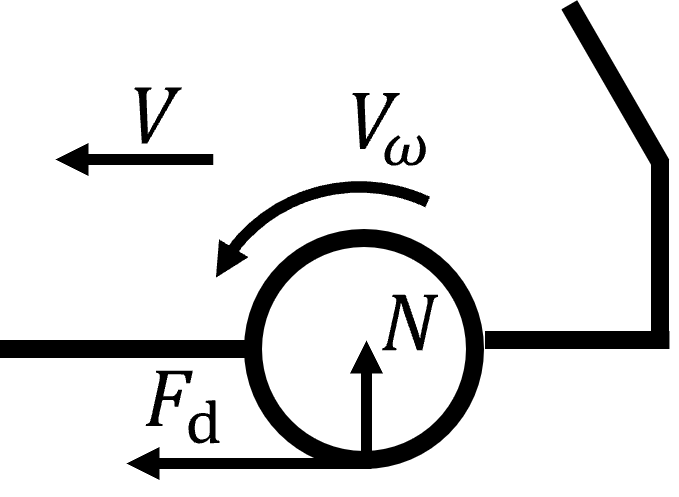
\includegraphics[width=\linewidth]{fig/2_car_model.png}
  \bisubcaption{車両モデル}{Vehicle model}
  \label{subfig:key-a}
\end{subfigure}\hfill
\begin{subfigure}{0.52\linewidth}
  \centering
  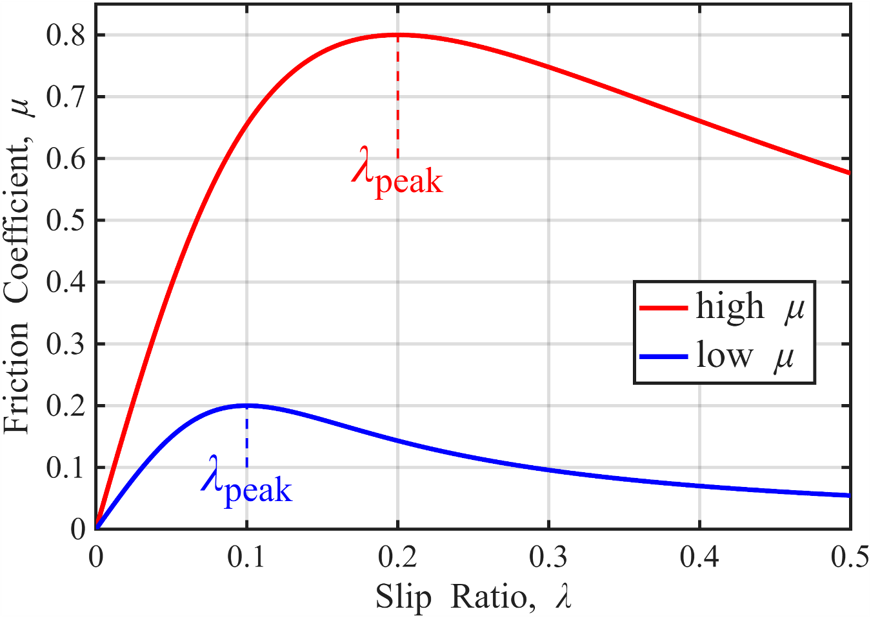
\includegraphics[width=\linewidth]{fig/2_mu-lambda_curve.png}
  \bisubcaption{$\mu-\lambda$曲線}{$\mu-\lambda$ curve}
  \label{subfig:key-b}
\end{subfigure}
\bicaption{車両およびタイヤの物理モデル}{Physical models of vehicle and tire–road interaction}
\label{fig:key}
\end{figure}



\begin{figure}[tb]
\centering
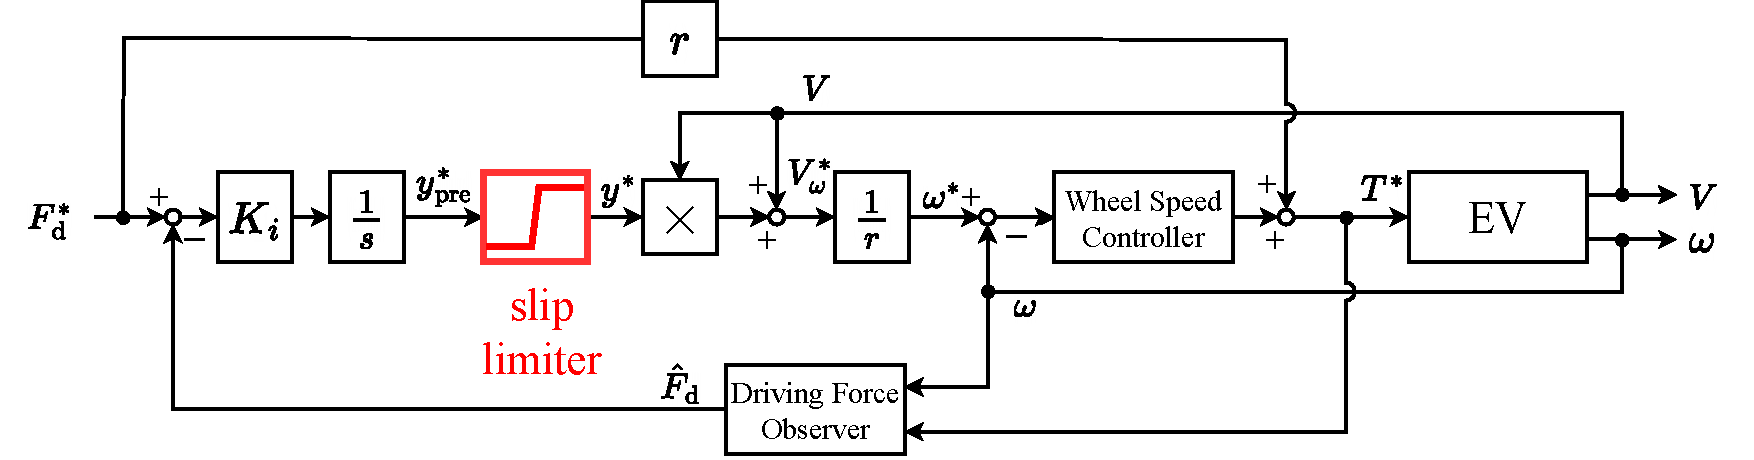
\includegraphics[width=\linewidth]{fig/1_DFC_circuit.pdf}
\captionsetup[bi-first]{name=図}
\captionsetup[bi-second]{name=Fig.}
\bicaption{駆動力制御(DFC)のブロック線図}{Block diagram of DFC}
\label{fig:1_DFC_circuit}
\end{figure}

\subsection{実験装置の概要}
実験装置の構成を記述する。

% ------------------------------------------------------------
% Figure template
% ------------------------------------------------------------
% \begin{figure}[tb]
%   \centering
%   \includegraphics[width=0.7\linewidth]{figure_name.pdf}
%   \bicaption{和文キャプション}{English caption.}
%   \label{fig:figure_label}
% \end{figure}
%
% 本文中の参照例：図\ref{fig:figure_label}に示す。

% ------------------------------------------------------------
% Two-panel figure template
% ------------------------------------------------------------
% \begin{figure}[tb]
%   \centering
%   \begin{subcaptionblock}[t]{0.48\linewidth}
%     \centering
%     \includegraphics[width=\linewidth]{figure_a.pdf}
%     \bisubcaption{和文キャプションA}{English caption A}
%   \end{subcaptionblock}
%   \hfill
%   \begin{subcaptionblock}[t]{0.48\linewidth}
%     \centering
%     \includegraphics[width=\linewidth]{figure_b.pdf}
%     \bisubcaption{和文キャプションB}{English caption B}
%   \end{subcaptionblock}
%   \bicaption{全体の和文キャプション}{Overall English caption.}
%   \label{fig:two_panel_label}
% \end{figure}

\subsection{数理モデル}
対象の数理モデルを記述する。

% ------------------------------------------------------------
% Equation templates
% ------------------------------------------------------------
\begin{equation}
  y(s) = G(s)u(s)
  \label{eq:example}
\end{equation}

% 本文中の参照例：式(\ref{eq:example})より，以下が得られる。

% \begin{align}
%   x_1 &= a+b，\\
%   x_2 &= c+d
%   \label{eq:align_example}
% \end{align}

% \begin{equation}
%   A =
%   \begin{pmatrix}
%     a_{11} & a_{12} \\
%     a_{21} & a_{22}
%   \end{pmatrix}
%   \label{eq:matrix_example}
% \end{equation}

% ------------------------------------------------------------
% Table template
% ------------------------------------------------------------
% \begin{table}[tb]
%   \centering
%   \bicaption{和文表題}{English table caption.}
%   \begin{tabularx}{\linewidth}{Xll}
%     \hline
%     Parameter & Value & Unit \\
%     \hline
%     Parameter 1 & $0.00$ & \si{unit} \\
%     Parameter 2 & $0.00$ & \si{unit} \\
%     \hline
%   \end{tabularx}
%   \label{tab:parameter_label}
% \end{table}
%
% 本文中の参照例：表\ref{tab:parameter_label}に示す。

\section{提案手法}
提案手法の概要，理論，設計手順などを記述する。

\subsection{手法の概要}
提案手法の基本的な考え方を記述する。

\subsection{設計方法}
設計式やアルゴリズムを記述する。

\section{検証}
シミュレーションおよび実験による検証方法を記述する。

\subsection{検証条件}
シミュレーション条件，実験条件，評価指標などを記述する。

\subsection{シミュレーション結果}
シミュレーション結果と考察を記述する。

\subsection{実験結果}
実験結果と考察を記述する。

\section{結論}
本稿で得られた成果をまとめ，今後の課題を記述する。

% ============================================================
% Bibliography
% ============================================================
\bibliographystyle{IEEJtran}
\bibliography{cite}

\end{document}
